% HCI Group Konstanz Seminar Template
% Version 1.1
%
% ATTENTION: This template was designed to fit the most common requirements for different types of reports (e.g., Seminar to the Project or Project Report). However, if you feel the need to add an extra component or layout feature please talk to your advisor. Please do not change anything on this template unless it is explicitly allowed or agreed with your advisor. However, it is allowed to add packages that do not alter the design/layout of this template.
%

\documentclass[10pt, paper=a4, parskip, oneside]{scrreprt}
\usepackage[T1]{fontenc}
\usepackage[utf8]{inputenc}
\usepackage{hciknseminar}
\usepackage[ngerman, english]{babel} % Spell checking (Using ngerman for german spell checking). The last language is the standard language for the document.
\addbibresource{bibliography.bib}

% =========== Title page ============
\title{Evaluating Gesture Based Teleportation Techniques For Immersive Virtual Environments} % Your title
\type{Master Thesis} % Seminar to the Bachelor/Master Project | Bachelor/Master Project Report
\author{Philip Oesterlin} % Your name
\studentno{01/993546} % Your student number
\group{Human-Computer Interaction} % Do not change this
\department{Computer and Information Science} % Do not change this
\advisor{Jonathan Wieland} % Your advisor
\reviewer{Prof. Dr. Harald Reiterer} % Do not change this
\date{\the\day .~\monthname~\the\year}

% ============= Abstract =============
\abstract{
    Locomotion in VR is an essencial feature for applications on a larger scale. However, with the increasingly popular option to use hand-tracking instead of controller inputs, there is not yet an established way to use locomotion. For this work the focus lied on teleportation based locomotion. To find results that are intuitive to the users, a gesture elicitation study was conducted. The study concluded in three different gesture systems. All of them include two stages: a targeting and a confirmation stage. This was not consistently included in the gestures found in excising literature but most of the study participants proposed a two step process. After implementing all three gestures into a prototype that allowed to compare the gestures in two tasks, a comparative study was performed. The results are not always conclusive but the best gesture seams to be a bimanual gesture that uses both thumbs and index fingers to consturct a triangle. This triangle is used for aiming and subsequently select a target point. To confirm the teleport location, the index fingers are pinched down to meat the thumbs. However, even though the gesture made the users perform the best on different metrics, the users did not always prefere this gesture even if it was working the best. A lot of users also liked a one-handed gesture that is using the index finger to target and the thumb to confirm the teleportation. However, with the current tracking technology, this gesture suffered some tracking and activation isses. If the tracking technology evolves further it still might be good candidate. The fact that it is a one-handed gesture would also be a benefit since it would improve the compatibility with more VR environments. However, with the current state of the technology, the triangular gesture is recommended.
}

% ============= Document =============
\begin{document}
% Title page
\maketitle
% Abstract
\makeabstract
% Table of contents
\tableofcontents
\addcontentsline{toc}{chapter}{Contents} % Add contents to table of contents
% List of Figures
\listoffigures
\addcontentsline{toc}{chapter}{\listfigurename} % Add list of figures to table of contents
% List of Tables
\listoftables
\addcontentsline{toc}{chapter}{\listtablename} % Add list of tables to table of contents
% Prepare chapters
\clearpage
\setcounter{romanPages}{\value{page}} % Update variable for roman pages
\pagenumbering{arabic} % Turn on page numbering again

% ============= Chapters =============



\chapter{Introduction}
The world of virtual reality (VR) is getting increasingly diverse. All kinds of tools and games are built, pushing the boundary of what is possible to create with current technologies. The computing hardware is also getting more powerful and more consumer-friendly. Standalone headsets that do not require a powerful computer linked over a cable are cheaper and can even be more immersive since the user does not has to keep track of the cable. The next step on the path of simplifying the experience could be to make it possible to use VR without controllers. They will still have their place for applications that require very acuate tracking, lots of different types of inputs or where it makes sense to hold something like a gun or paintbrush. Many experiences do not require this, however. Especially for applications and tools used to collaborate, enabling users to enhance their communication with gestures might be helpful. Use-cases like this are where hand-tracking will allow the implementation of immersive, natural interfaces. This can allow anybody to just put the headset on and start interacting with the virtual world without first being told how to grab something or how to activate a button, as shown in figure \ref{fig:example}. However, as stated before, the interactions do have limitations in terms of accuracy and their number of inputs and are a challenge to get right. Users will first apply the mental model built during decades of experience using their hands in the real world. Differences between the real and the virtual world might therefore make the experience less immersive than if the user were using a controller where there is no previous knowledge. This raises the question of what to do if the virtual world allows users to do more with their hands than in the real world. 

\begin{figure}[!ht]
    \centering
    \includegraphics[width=\textwidth]{figures/examplegestures.png}
    \caption{Example of users interacting with objects in VR using hand-tracking. \cite{Han}}
    \label{fig:example}
\end{figure}


One simple way where VR technology can expand on what is possible in the real world is scale. The area a user is physically able to explore and walk around comfortably is limited. For most casual users of VR, that might be the size of their living room. In VR, this is not a limitation. There, a user can be given the ability to fly, teleport or use any number of so-called locomotion techniques to increase their level of comfort and allow them to go wherever they want. While not completely understood, the disconnect between the real world's movement and VR is likely one source of motion sickness. This makes locomotion a necessary mechanic to implement in large scale VR experiences and a very divisive one since it can impact the users' immersion and level of comfort a lot. VR experiences only offering continuous locomotion can, for some users that are more prone to get motion sick, only be usable for a few minutes, only with a limited field of view or not useable at all. On the other hand, users that are used to continuous navigation do not get motion sick as quickly or even at all report being frustrated by having to use another, less immersive locomotion mechanic that might get in the way a lot more. So while teleportation based locomotion is not needed for everyone, it allows most people to at least use large scale VR experiences comfortably without getting sick. This makes it the first and sometimes only mechanic that is implemented, and so it should be as well understood and implemented as possible. Especially when in combination with hand-tracking and gesture-based teleportation, there is only minimal research done so far.

This work expands the previously done research on how locomotion or, more specifically, teleportation should work using hand-tracking. Teleportation is the most popular form of locomotion in VR. When using controllers, locomotion is usually controlled using a joystick or button, and even though there are slight differences between each game, you can usually figure out quickly how to control it. Without controllers, there is no conventional way to control teleportation. The user can also not easily hit all the buttons until some feedback can lead them in the right direction. VR applications based on hand-tracking will, therefore, still have a learning curve for new users. If there is a standard way to use teleportation established, it should be based on research. 

% goal of the thesis

% maybe structure

% bilder





% Introduction
Enabling simulated movement in virtual environments is not a new problem. 
The techniques that allow the user to move their viewpoint require special attention in regards to immersiveness, cybersickness, ergonomics and path integration, concepts explained in the following chapter.

% TODO: why sections are chosen


\section{Motion Sickness}\label{motion-sickness}

The phenomenon known today as motion sickness predates modern technology
by millennia and even Hippocrates wrote about it. The word ``nausea'',
the main symptom of motion sickness is also derived from the Greek word
for ship ``naus''. \cite{Golding} It is a very
unpleasant feeling and was even used as a legal punishment in the 19th
Century \cite{Reason}. The source of motion sickness is
well understood because there is a lot research from military agencies
since they had to transport a lot of soldiers by ship and needed them to
be healthy when they reached their destination
\cite{Johnson}. After the invention of the first flight
simulator, the term simulator sickness was coined. Simulator sickness is
a form of motion sickness that can occur when training pilots in
simulators \cite{Johnson}. With the rise of head mounted
displays and VR technology, motion sickness got another subcategory:
virtual reality sickness, also known as cybersickness. It is distinct
from simulator sickness because the symptoms are not as much related to
the Oculomotor system (for example eyestrain, blurred vision, etc) but
rather disorienting. The severity was found to be about 3 times greater
than simulator sickness. This might be because the VR systems are more
immersive than a flight simulator that relies on traditional displays
\cite{Stanney}.\\Because cybersickness and simulator
sickness are different, there needs to be a separate evaluation method
for the two phenomena. According to Stone et al. \cite{Stone} this is because the
weighted scale of the simulator sickness questionnaire does not
translate well to the VR environment. This is improved with a new
weighting scale proposed by Stone et al. \cite{Stone} but a new questionnaire
specifically created for cybersickness generates the best results.
However the simulator sickness questionnaire is often used in reached
anyway. This only has the benefit that the results are easy to compare
but there are significant tradeoffs in regards to accuracy.

\subsection{Cybersickness}\label{cybersickness}

As discussed before, cybersickness is a form of motion sickness. It can
result in a range of symptoms including nausea, vomiting,
disorientation, headaches and eye strain
\cite{LaViola}. This is a serious problem and needs to
be taken into account when developing VR systems.

% TODO: indent direct quote
The actual cause of cybersickness is not
known and the underlying physiological responses uncertain. According to Davis et al. \cite{Davis} The three
most prominent theories for the cause of cybersickness are poison
theory, postural instability theory and sensory conflict theory.

\begin{itemize}
\itemsep1pt\parskip0pt\parsep0pt
\item
  Poison theory: survival mechanism that induces vomiting and nausea to
  remove poison from the body if the brain detects sensory input like
  hallucinations.\\
\item
  Postural instability theory: a loss of postural control causes
  sickness\\
\item
  Sensory conflict theory: symptoms are created if there is a conflict
  between the vestibular and visual senses. For example if a user is not
  moving but their avatar in VR is.
\end{itemize}

Unfortunately all three theories have low predictive power and fail to
explain some key aspects of cybersickness~\cite{Davis}.

One way to reduce cybersickness is to break the optical flow the user
perceives using different kinds of techniques
\cite{Bhandari}. Optical flow is a phenomenon that
allows an observer to gather information about the motion of objects and
give the observer a sense of presence \cite{Gibson}.

\section{Locomotion in VR}\label{locomotion-in-vr}
% TODO: cite
The ability to move the players avatar in the virtual environment is
called locomotion. It is required for many applications or games that
take place on a larger scale. Without locomotion techniques VR would be
very inaccessible. A user would need a giant tracking space, which is
not possible in most homes and also the technology to track the users
headset would have to work over that amount of space. Locomotion is also
needed even if you could walk everywhere in your space, since it can
also be a convenience or accessibility feature in combination with a
seated experience. Getting the locomotion mechanics just right, will
also improve other interactions and user satisfaction in general. Moving
to a different virtual altitude would also not be possible without some
technique that can simulate the player walking up stairs. Otherwise
every user would have to have stairs in their tracked space. The
implementations of locomotion techniques can be very divers and so there
is a wide range of categorizations schemes.

Luca et al. \cite{Luca} collected 109 different locomotion techniques from academic
sources, social media and popular VR games. The result is a public
database of methods that can be filtered and compared. Some of the
methods are in a preliminary state and not fully implemented or
evaluated but in general the database is a great resource. There are only 8 results for hand-tracking
are some of them are falsely categorized.

\subsection{Locomotion using controllers}\label{locomotion-using-controllers}

Boletsis et al. \cite{Boletsis} categorized the four
prevalent locomotion techniques into:

\begin{itemize}
\itemsep1pt\parskip0pt\parsep0pt
\item
  Room-scale-based: uses physical movement, translates movement from the
  read world one to one into VR. continuos movement, unlimited range.\\
\item
  Motion-based: uses physical movement for example swinging arms or
  walking in place. Continuos movement, unlimited range\\
\item
  Controller-based: The uses controller input like a joystick to move.
  Continuos movement, unlimited range.\\
\item
  Teleportation-based: the viewpoint is instantly moved to a new
  predefined location. Non-continuos, unlimited range
\end{itemize}

The room-scale-based techniques are limited to the size of the tracking
space so they are not flexible enough for a general use case. If the
task allows it, it should however be the preferred locomotion technique
because it results in the best immersion while also keeping
cybersickness to a minimum.

Controller-based techniques could be adapted into a hand-tracking
environment, the continuos nature of the movement, without some kind of
a physical representation of the movement performed by user however
would make it prone to create motion sickness.

Motion-based techniques are very dynamic because of their physical
nature. That makes them hard to track with current hand-tracking
technology. They also made users tired the fastest.

For those reasons the scope of this work will focus on only
teleportation-based techniques to give results that as widely useable as
possible and accessible to the most amount of people without inducing
cybersickness.

\subsubsection{Teleportation-based locomotion}\label{teleportation-based-locomotion}

Teleportation is one of the most used locomotion techniques. Each
implementation can be slightly different in the way it is integrated
into the virtual environment but the core mechanic allows the user to
move the viewpoint to points on the map using some ray casting system.
There is usually a limit to the teleport distance and sometimes the user
is only allowed to select predefined locations as targets. The technique
is categorized as non-continuos movement with unlimited range. Since not
only the xy coordinates of a target location can be chosen but also
points at different altitudes, the method has 3 degrees of freedom.

The research from Clifton et al. \cite{Clifton} shows that on average teleportation
causes less cybersickness than continuos navigation, however, there were
some people (38\%) that had the opposite reaction.
Clifton et al. conclude that there should always be multiple locomotion
methods to choose from. The researchers theorize that the cause of the
cybersickness might be that some people are more sensitive to the
immediate displacement used by teleportation-based locomotion. If the
participants experienced the virtual environment while sitting or
standing did not make a cause a meaningful change in the reported
effects, only that there seems to be slightly worse cybersickness from a
seated experience. 

However, teleportation is also not the perfect solution. 
The lack of optical flow between locations is great to minimize
cybersickness, but it also introduces limitations. 
Path integration, a process where the brain updates the current position
continuously using information from different senses. Visual, vestibular
and proprioceptive sensory input are continuously integrated and create
a rough estimate of the distance traveled. \cite{Bhandari}

Bhandari et al. \cite{Bhandari} found that this can be improved by allowing some optical
flow between teleport points without creating higher levels of
cybersickness. This can be achieved by using a technique the researchers
call ``Dash''. It translates the user at a constant velocity from the
current point to the target. This creates a short transition period that
takes a maximum of 1.1 seconds over a maximum distance of 11 meters in a
virtual environment at real world scale. Previous research indicates
that the duration and speed do not impact the resulting effect a lot
\cite{Bowman} but these values where picked after some
internal testing. Using this technique users where able to move back to
a starting point after teleporting away much more accurately without any
landmark or context clues. 

An interesting problem with teleportation-based locomotion is that is
was found to be the least immersive technique out of the four types
categorized by Boletsis et al. \cite{Boletsis}. This
could improve using hand-tracking because the users can use their own
hands and that might be more immersive for some people. % TODO: (maybe include in hypotheses)


\subsection{Locomotion using hand-tracking}\label{locomotion-using-hand-tracking}

Only a rather limited amount of research was done about locomotion using hand-tracking even though natural human-computer-interaction using gestures is not a new field of study. Schäfer et al. \cite{Schafer2021} conducted a study using very basic gestures. In their virtual environment the simplest gesture only requires the user to point a finger in a forward direction to produce a visual ray in the respective direction. If this ray intersects with a valid teleportation location, a little reticle appears on that point. This marks the teleportation target. If the user keeps their hand still for 1.5s the teleportation to the target location is performed. Schäfer et al. also implemented other variations on this gesture:

There are two ways to select a location:
\begin{itemize}
  \item point index finger to select a location, named the index method
  \item use the normal vector of the palm to select a locomotion, named the palm method
\end{itemize}

There are also two ways to confirm a target:
\begin{itemize}
  \item the user keeps their hand still for 1.5s
  \item the user uses a second hand to confirm the location. For this a method was implemented where the left hand can first rests in a neutral position while a target is selected with the right hand. To confirm the teleport location, the user performs a pointing gesture with the second hand while keeping the right hand on the target.
\end{itemize}

The results of a user study conducted by Schäfer et al. \cite{Schafer2021} show the method using a one-handed palm gesture achieved the highest user satisfaction ratings (90 of 100 possible points). However, there appear to be some problems with the implementation. The authors noticed that bimanual methods loose tracking more often so this might influence the immersion and user satisfaction results. Another tracking issue was also found with the index method. The noise in the tracking data appears to frustrate users when trying to select a target. The tracking issues make it seem like the one handed palm gesture was only preferred by users because users found the unreliable tracking frustrating. This is also confirmed by the NASA-TLX results. The users reported to be more frustrated with the methods influenced by the bimanual tracking issues and the index finger tracking noise. The method influenced by both types of issues got the worst score. 

\begin{figure}[hbt!]
  \centering
  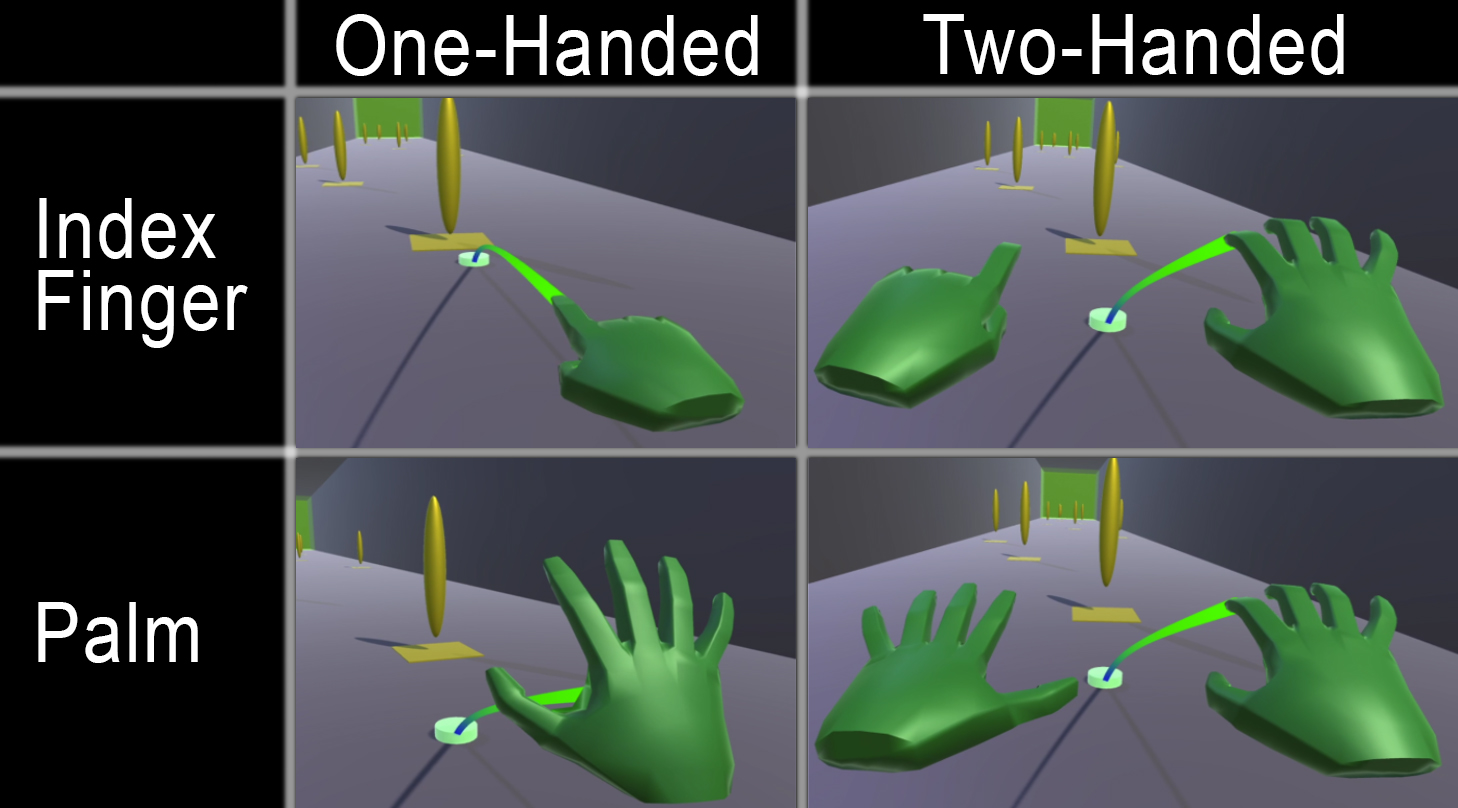
\includegraphics[width=\textwidth]{figures/1h vs 2h gesture study.jpg}
  \caption{Gesture types included in the study from Schäfer et al. \cite{Schafer2021}}
  \label{fig:1vs2}
\end{figure}

The one-handed palm method was the gesture that had the least amount of tracking issues since it was single handed and was not only using the index finger for target selection. This is result is surprising since the gesture violates multiple principles for a comfortable gesture detailed in \ref{ergonomics}. However, in a short study this might not influence the user satisfaction too much. The negative effects of uncomfortable gestures might not be noticeable after only using the gesture for the short duration of the study, so that the users are not experiencing the longer term effects. 

The one-handed palm method, the gesture with the highest usability score, also has other limitations. It would get even more uncomfortable when trying to teleport to some elevated targets. This would put a lot of strain on the wrist, which is one of the most problematic areas. The automatic confirmation of a target used also does not provide any feedback to the user like the bimanual methods do. Some of these issues can be improved on but it seems like the tracking is the most important issues to solve for now and that this is can only be solved using different gestures that enable more robust tracking with lest noise.

For traditional locomotion using controllers, the locomotion database from Luca et al. \cite{Luca} is a great resource. It includes solutions, that are user tested, established in the industry as well as more experimental ones. However, when filtering the locomotion database for techniques that are categorized to use hand-tracking only 8 results are presented.
The results that are relevant for this paper are:

\begin{itemize}
\item
  Hand Close: a gesture for continuos movement. Seems to have problems
  with cybersickness (25\% of study participants had to
  abort the 90 minute test). \cite{Huang}
\item
  Finger Run: two-handed gesture for continuos movement, the only
  resource is a video on a game development account that mostly posts fun
  prototyping ideas. \cite{Beauchamp}
\item
  Walking stick: a gesture instantiates a walking stick, that can be
  used to move the user in relation to the sticks touch point on the
  ground. This is only a preliminary database entry though and this is
  not a great solution for big distances or different altitudes. % TODO: cite
\end{itemize}

The categorizations seem to have some issues and so going through all
109 techniques, a small list of more gestures can be found that might work using gestures:

% TODO: integrate
\begin{itemize}
\itemsep1pt\parskip0pt\parsep0pt
\item
  World in miniature: manipulate player position on a miniature version of the environment
\item
  Cloudstep: small teleportation steps using a joystick
\item
  Dash Pointing: fast, continuos step in the direction of the controller with limited field of view
\end{itemize}

 % TODO: cite

Problems when trying to translate other methods into an environment without controllers:

\begin{itemize}
\item
  limited tracking space for hands: Controllers can still detect button
  presses and orientation changes if they are out of the tracking
  region, like behind the body. The hand-tracking system has no idea
  what the users hands are doing if they are out of view or obscuring
  each other.\\
\item
  limited accuracy: Hand-tracking is much less accurate with current
  technology. This might improve in the future though.\\
\item
  Hand-to-hand interaction is confusing the hand-tracking system\\
\end{itemize}

\section{Gestures}\label{gestures}

Emerging technologies enable new human-computer interaction techniques. Gestures are a core part of human communication so it only makes sense to adapt them for user interfaces. However, gestures are not new only the technology to be able to detect them is. There are also sources of information from other fields of research, like research on sign language, that can be of use to create gestures that are comfortable and intuitive.


\subsection{Gesture Detection}\label{gesture-detection}

The most accessible hand-tracking hardware for virtual reality today is
the Oculus Quest 2 VR headset. It has hand-tracking build in, which can
be accessed using the Oculus SDK in Unity. The exact technology the
Oculus Quest device uses is not known. However it can be speculated that
Oculus is using a variation of the research done by Han et al \cite{Han}. The
Oculus Quest only has monochrome cameras and only a very limited amount
of processing power, which correlates with the limitations addressed by
Han et al. \cite{Han}. Like the Oculus Quest, the
unnamed headset in the paper has 4 cameras. They are positioned on the
headsets corners, all facing in slightly different directions to cover a
120° area in front and below the headset. The areas the individual
cameras can see overlap in some places so that in the most important
areas the hands are visible for at least 2 up to 4 cameras. The
tracking system works by first detecting the hands in the camera streams
using a CNN architecture optimized for efficiency named DetNet. The
network can simultaneously localize and classify the hands which
combines two steps into one. Next, a network called KeyNet takes the the
cropped camera images and outputs 21 coordinates that match key points
of a human hand. The network architecture is optimized to reduce jitter
and consistency when moving between overlapping camera areas. This is
done using extrapolated points as an additional network input. The
output is suitable for basic interactions and certainty impressive for
real time processing on mobile hardware but there are definite
limitations. Since Hand-to-hand occlusions and interactions were not
part of the training set, the output has problems with complicated
poses.

% TODO: cite schäfer 3.3 capturing gestures

\subsection{Future Technology}\label{future-technology}

Current technology has some major limitations when tracking hands.
Hand-to-hand interactions, self-contact and occlusion come to mind.
Smith et al. \cite{Smith} created a system that takes in high resolution data from
124 cameras capturing uniformly lit hands. The images are turned into a
mesh so detailed its basically indistinguishable from the original
hands. The pose of two hands and even the texture is captured without
any artifacts. This process is very complex and it takes minutes to
render per frame so it will take some optimization until detailed hand
models like this could be included in a VR environment. However, this is
the direction that technology will go, even if it will take some time.
That means that even if hand-to-hand interaction is not able to be
reliably tracked currently, it could be in the future.

\subsection{Intuitive and comfortable gestures}\label{ergonomics}
For the design of a hand gesture vocabulary, the first consideration might be how well the gesture can be identified. However, gestures that are easily recognized may not be intuitive and easy to perform by the user. According to Stern at al. \cite{Stern2006} there are three factors that all should be maximized when choosing a gesture: intuitiveness, comfort and recognition accuracy.

Stern et al. define intuitiveness as the cognitive association between a command or intent and its physical gestural expression. Experiments that trying to find universal gestures for a virtual reality environment were also done by Pereira et al. \cite{Pereira2015}. The in the experiment 34 participants were asked to come up with gestures for common HCI tasks like. % TODO: sample
This resulted in over 1300 different gestures for 34 tasks. However, only 84 gestures were chosen by 3 or more subjects and some of them for different tasks. Expecting the user to intuitively guess the same gesture that the developers of the virtual environment intended therefore seems unrealistic. Constructing a gesture that requires no introduction or tutorial is therefore also not the goal of this paper.

The research of Ardito et al. \cite{Ardito2014} also supports this. They compare trying to design universal gestures to problems that arose with visual languages in the past. They predict that trying to use the same gesture vocabulary over a range of applications and devices is likely to fail. 


As a measure for comfort, Kölsch et al. propose a method that distinguishes between a pose of some joint or body part and the user compensating using other joints to relieve strain. A compensation for a pose that requires the users head to be tilted onto its side might be to keep the head upright relative to the body but bend the torso to the side. To find the optimal comfort zone of a posture, Kölsch et al. \cite{Koelsch} measure how users compensate or if they execute the pose without compensating. 

There are also other methods that rely on biomechanical models and physics simulations to measure how comfortable a gesture is but they are prone to errors \cite{Stern2006}.

Another source of knowledge to source information from regarding gestures are sign language interpreters. They might spend more than 20 h per week signing, however, they also often suffer from hand pain and fatigue while gesturing for long sessions. This would also be a risk for prolonged sessions in virtual reality that is using hand-tracking gestures. Rempel et al. conducted a study with experienced sign language interpreters to find the discomfort level associated with signing selected hand postures, motions and characters \cite{Rempel2014}. 

Rempel et al. \cite{Rempel2014} collected findings and summarized:
\begin{itemize}
  \item Hands should be near the midline of the body and not further apart than the shoulders. They should be near the height of the elbows and close to the lower chest, so that the shoulder muscles are not tense. 
  \item Sustained elbow flexion of more than 90 degrees should be avoided.
  \item The most comfortable postures were between neutral and 45 degrees of pronation (palms rotated toward ground). Repeated full rotations to palm up (supination) or palm down (pronation) should be avoided.
  \item Gestures that included movement of the elbow or shoulder were more comfortable than gestures with just finger movements.
  \item The more comfortable gesture motions were up-down hand movements performed with motion at the elbows or side-to-side hand movements with motion at the shoulders. 
  \item the most comfortable hand gestures were with the wrists straight and the fingers slightly flexed or in a loose fist.
  \item The least comfortable gestures were those involving wrist flexion; discordant adjacent fingers; or fingers extended.
  \item The position of the thumb did not appear to have a large influence on comfort.
\end{itemize}



\section{Usage in Games}
In the games industry there are some examples of gesture based movement present. The gestures used are probably tested and evaluated internally but there is currently no information published how well they work statistically, if they are ergonomic or usable. That means that for now, they can only be compared on a basis of personal experience. 


\subsection{Vacation simulator}
Vacation simulator \cite{VacSimOculus} is a VR simulation game, the sequel to the popular game Job Simulator. Released in 2019 by Owlchemy Labs, it was updated in late 2020 to enable hand-tracking support \cite{VacSimBlog}. The game has a lot of intuitive mechanics that translate very well to hand-tracking, like its use of a physical backpack as a game menu. The teleportation system is very easy to control but comes with the limitations that the user can only teleport to large predefined areas. Therefore, the gesture does not need to be very accurate. The user only needs to "pull" the target closer using a gesture shown in \ref{fig:pull}. 

\begin{figure}[hbt!]
  \centering
  \includegraphics[width=\textwidth]{figures/vacsim.jpg}
  \caption{Selecting a target area and confirming teleportation in Vacation Simulator}
  \label{fig:pull}
\end{figure}

This works well for this use case, where the teleportation does not need to be accurate. During testing, this was never a problem and might have even be more intuitive than using a controller because its so easy to remember and control, whereas some unexperienced users sometimes seam to have problems with the activation of controller based teleportation using the joystick. 


\subsection{Elixir}
One of the first hand-tracking titles for the Oculus Quest was Elixir. A short demo game where a user is allowed to explore a magic chamber. The chamber could be explored using Room-scale-based movement if the user has a large enough play space, however there is also a teleportation system included. It works using a bimanual gesture. Both hands form a triangle using both thumbs and index fingers. This can be used to target a point on the floor. The teleport resolution is limited to a grid system on the floor. Once selected a tile on the floor lights up. To confirm the tile as the target location, the user pinches the respective thumbs and index fingers together. The viewpoint is the instantly moved to the new location.

\begin{figure}[hbt!]
  \centering
  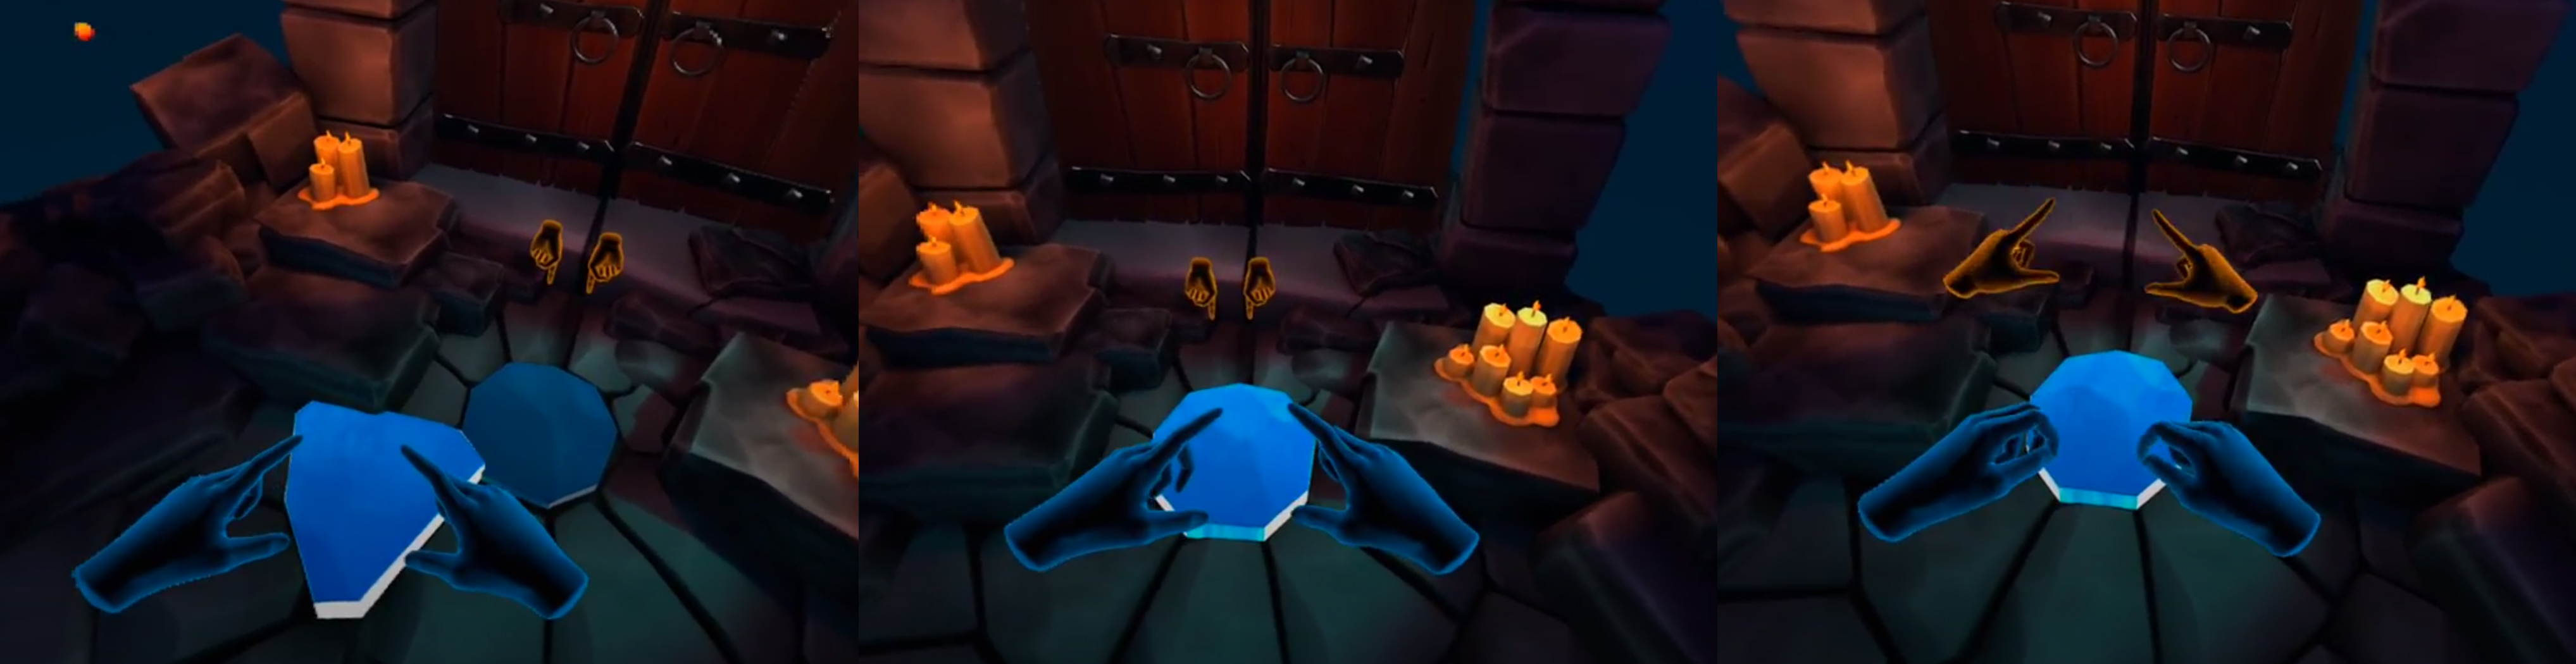
\includegraphics[width=\textwidth]{figures/elixir.jpg}
  \caption{Selecting a target and confirming teleportation in Elixir}
  \label{fig:elixir}
\end{figure}

The system does not allow the user to teleport to any point which is technically a limitation. However, in practice it makes the tracking more stable while sill allowing good control. Having a gesture to confirm makes the system feel controllable. 


\subsection{Waltz of the Wizard}
In the fantasy game Waltz of the Wizard \cite{WaWizOculus} by the Studio Aldin Dynamics \cite{Aladin}, the user can learn spells and have fun manipulating the environment. The game has been updated to support hand-tracking \cite{WaWizBlog}. This also includes an adaptation of the custom teleport system the game used in its original version called Telepath \cite{WaWizTelePath}. To move, the user draws a path on the floor. This path is broken up into sections. The system moves the users viewpoint from one point to the next, while dynamically adjusting the pause between the teleport steps. This allows the user to pick up objects while walking, or increase the walking speed by swinging arms. In contrast to the other systems, Telepath can be used to move to any point, without the limitations of the other systems. It does not require a grid system on the floor and is not limited to only specified teleport points.

\begin{figure}[hbt!]
  \centering
  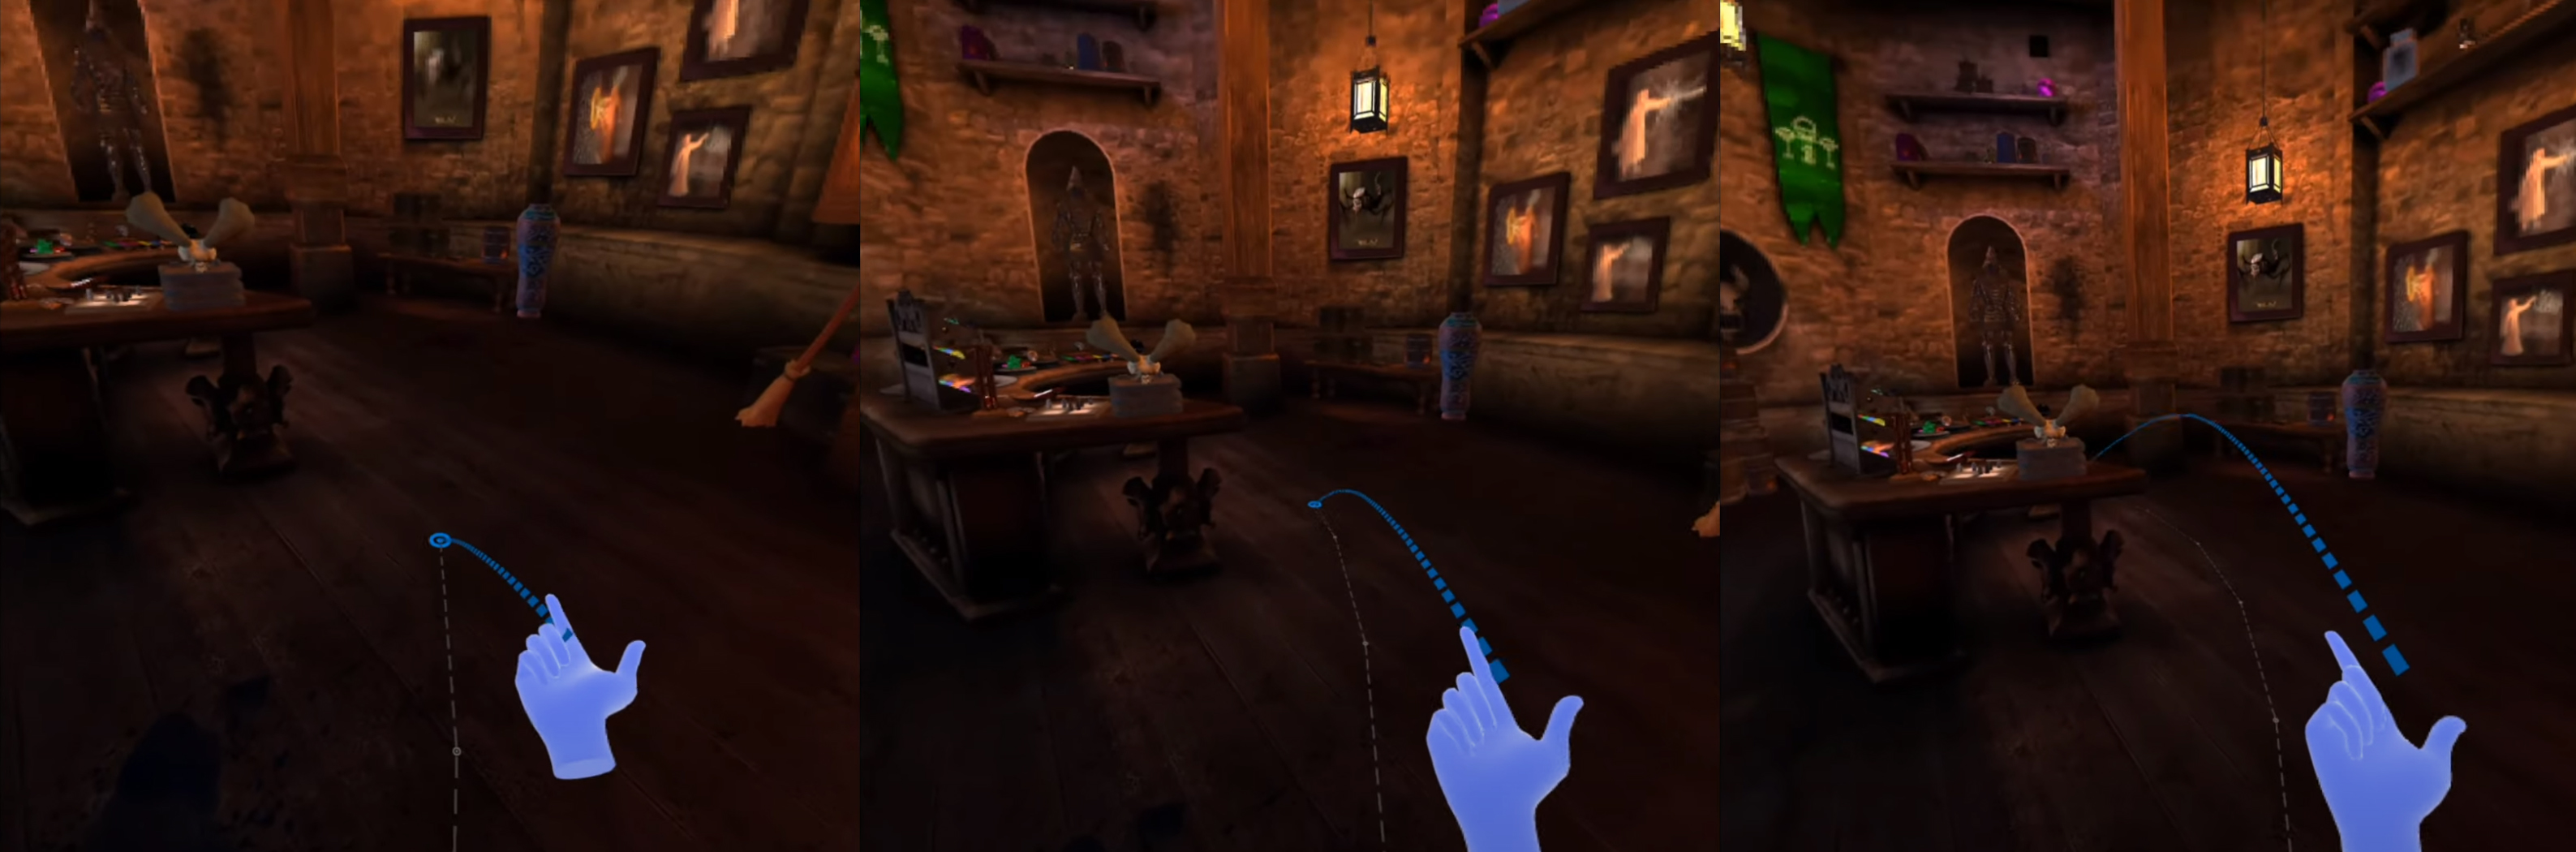
\includegraphics[width=\textwidth]{figures/waltz of the wizard - point.jpg}
  \caption{Telepath gesture: draw walking path using index finger}
  \label{fig:telepath}
\end{figure}

During testing, the Telepath system did not induce cybersickness even though the movement did required a short period of getting used to. The accuracy of the gesture recognition system left a lot to be desired however and the experience was frustrating at times. Ergonomics are also a point to criticize, size the gesture strains the hands quite uncomfortably even after only a short test of 20 minutes. Drawing a path still seams to be a promising idea and might enable high levels of immersion and allow the brain to perform path integration while not inducing cybersickness. Short bursts of quick movements have also been analysed by Bhandari et al. \cite{Bhandari}. It produced promising results regarding cybersickness and and path integration. 

\section{Study Designs}
For the comparative user study, it is helpful to look at methods used in the literature. 


The study designed by Bozgeyikli et al. \cite{bozgeyikli} compares 3 locomotion systems in the same environment. A gesture based point and teleport system, a walk in place system and a system using a joystick. The later two are continuos locomotion systems, while the first is a teleportation system. The environment was designed to be very basic to keep the focus on the locomotion. It includes 6 target points with a 0.6m radius placed on the ground. There are also 21 obstacle pillars scattered around in the environment. The task for the users is to move to a highlighted target, to wait for 3 seconds on the point and then move on to next point.

The independent variable in this study and all others described here, is the gesture tested. The dependent variables are the time to reach destination points, the number of collisions with the obstacles and the results of the usability survey. 
However collisions can only occur while using the two types of continuos locomotion. 



The study designed by Schäfer et al \cite{Schafer2021} also uses a primitive environment in the form of a long corridor to reduce the wow effect for first time users. The environment includes ten markers spaced out along the corridor. The participants task is to touch all the markers while traveling through the corridor. To explain the gestures an introduction is added to the study in form of a tutorial video.

In this case the dependent variables are the task completion time, the number of teleports, the number of times the tracking is lost and the results of a usability survey.


The study designed by Caggianese et al. \cite{Caggianese} uses a detailed, immersive environment as shown in \ref{fig:path}. It includes a very long path way of 343m with distractors along the way. The users task is to follow the path from start to end. 

The dependent variables in this case are efficiency and effectiveness of each gesture. Efficiency is derived from completion time. The effectiveness is derived from performed errors, locomotion interruptions and tracking errors. There are also five questionnaires (SSQ, SAM, SUS, SEQ, NASA-TLX) for each participant to fill out after each run.

\begin{figure}[hbt!]
  \centering
  \includegraphics[width=\textwidth]{figures/path-of-study.PNG}
  \caption{Caggianese et al. \cite{Caggianese} Task}
  \label{fig:path}
\end{figure}


The study designed by Bhandari et al. \cite{Bhandari} uses an extremely basic environment with only a ground plane and a sky above. This is so that the brain is not able to compute path integration from context clues. The users task is to move to a self-selected target point in the distance, to turn around and then to try to hit the start point again. A diagram is shown in \ref{fig:backAndForth}.

\begin{figure}[hbt!]
  \centering
  \includegraphics[width=\textwidth]{figures/back-and-forth.png}
  \caption{Bhandari et al. \cite{Bhandari} Task}
  \label{fig:backAndForth}
\end{figure}

In this case the dependent variable is how large the distance $a$ is. From this value it is derived how well the brain is able to grasp how far the traveled distance was and how repeatable the gesture is.

\section{Conclusion}
The research done so far has not produced a conclusive answer how to teleport using hand gestures. It is even disputed if such a solution is possible to find at all. The game industry has found some methods for different use cases and environments, there is however no way to compare them in a controlled environment, since they are each implemented in their respective games. The goal of this project is therefore, to create a test environment to compare methods from the literature and selected games in a standardized way. 


\chapter{Gesture Elicitation Study}
In order to get an overview over what kind of gesture systems can be considered intuitive a small Gesture Elicitation Study based on the research of Villarreal-Narvaez et al. \cite{elicitation} was performed. This was an important first step in the selection of the gesture systems to conduct further research on. 

\section{Study Setup}
The participants were instructed to come up with teleportation techniques and to explain them in detail. One and two-handed gesture systems are allowed. To understand the limitations of hand-tracking the subjects were wearing the Oculus Quest device with hand-tracking enabled. This way it is easy to tell which gesture is tracking well and what is not detected by the tracking cameras. A simple environment with only a plain on the bottom, the skybox and the users tracked virtual hands was used. The environment was created so that the focus lies on the hands and the gestures. During the study, the headset was connected to the WebSocket relay application. Using a simple web interface, the study operator could connect to the WebSocket as well and send commands to the headset. Pressing the "Save" button on the web application records the current gesture. It is sent to the main server application to allow the detailed analysis of gestures in the Visualizer after the study. This was done because it would not have been realistic to record everything the participant does with their hands. The WebSocket then allows the communication with the headset with very little delay, so that important gestures can be saved when the participant is trying something out. The Visualizer also allowed the operator to check if the recording of the gesture data worked during the study. The gesture data was backed up after each participant run. The conversation between the operator and the participants was also recorded on video for analysis. The sessions lasted on average about six minutes.


\section{Results}
$28$ different gesture systems were collected from the video and gesture snapshot information, with five systems appearing twice. Nine gesture systems are not usable for the comparison since they are either not strictly teleportation systems or because they can not be compared to other teleportation methods like a system using a minimap or a type of proxy system. Out of the usable 19 systems, six use a bimanual approach while 13 use one hand. This trend to one-handed gesture systems was also explicitly called for by two participants that expressed some possible downsides of bimanual systems. The participants reported more physical effort and not being able to carry something in one hand while teleporting as a disadvantage.

The usable gestures can be categorized into three large groups of similar gesture systems. 

The largest group of systems are all using at least one hand with the index finger extended to use as a pointing device. In total this method was proposed eight times. One gesture is also using an extended middle finger to make the gesture more distinct (\ref{fig:index2}) but the targeting system otherwise works the same. Six times the system was proposed to have a confirmation step before the teleport is actually performed. According to the participants, this should work by using a "finger gun" type gesture where the thumb is first extended and is then tapped against the base of the index finger to confirm the teleport location as seen in \ref{fig:index}. One user also proposed to gesture an "air tap" with the extended index finger. However, he expressed some concern about the accuracy, since moving the finger to confirm could impact the target selection. Twice the second hand was used as a confirmation step but did not influence the targeting system using the pointing hand.

\begin{figure}[!ht]
    \centering
    \includegraphics[width=0.5\textwidth]{figures/double index.jpg}
    \caption{Pointing gesture with index and middle finger extended.}
    \label{fig:index2}
\end{figure}

\begin{figure}[!ht]
    \centering
    \includegraphics[width=\textwidth]{figures/index.jpg}
    \caption{Index finger pointing gesture with two stages.}
    \label{fig:index}
\end{figure}


The second biggest group of gestures was named six times. All gestures are using a single, open hand with some kind of confirmation step as shown in \ref{fig:palm2}. Four times closing the hand to a fist was proposed as a confirmation step, with the others quickly tapping the index finger and the thumb together to select the target. Another difference between the systems is also the direction the open hand is pointing towards. Four times a ray would start as the normal vector of the palm of the hand, once out of the middle finger. One other system proposed to have the palm upwards, with an arc used as the targeting visualization. The arc would curve in the direction of the middle finger and could be manipulated by changing the height of the hand. Holding the hand up high makes the arc go further and would therefore allow teleports over a larger distance.

\begin{figure}[!ht]
    \centering
    \includegraphics[width=\textwidth]{figures/palm.jpg}
    \caption{Palm gesture with two stages.}
    \label{fig:palm2}
\end{figure}

A third group is named five times and is using only bimanual systems that use a targeting system where the selection vector is produced by some kind of "rangefinder", the user is looking through. This could be a triangle formed by touching both index fingers and both thumbs together. This was proposed four times. Another proposed option is a "diamond" form formed by touching all fingers to their equivalent finger of the other hand. This forms a hole that can be used to look through. This was proposed twice. All but one system also include a confirmation step that is performed by closing other fingers to a half fist or pinching the hole together.

Other honorable mentions are:
\begin{itemize}
    \item Wrist mounted laser pointer
    \item Pointing using a thumb
    \item OK-Gesture with using the middle finger to point, confirmed when opening the sign
    \item Throwing a teleport ball to a target
    \item Drawing a circle in the air that will become the new viewport
\end{itemize}

They were all mentioned only once but could also be interesting to investigate.

\section{Discussion}
The results appeared promising for the usability study since most of the intuitively proposed gesture systems by the test subjects are very similar or at least follow the same ideas as the gesture systems found in previous works. There are some notable exceptions however. Only 3 out of 19 gesture systems proposed by the participants did not include an explicit explanation for a confirmation step. This made it apparent that the users would not expect a gesture system based on dwell time like proposed by Schäfer et al. \cite{Schafer2021}.
\chapter{Implementation Overview}
\label{cha:ImplementationOverview}

\section{Gesture Recognition}
A big problem early on in the development of the detection algorithm was how different human hands can be. The detection had to be accurate enough to decide between stored gestures based only one different finger, while staying flexible enough so a user could adjust their hands posture or simply have their own interpretation of the gesture. This turned out to be quite difficult to implement. The final implementation took the following approach to improve the detection accuracy and speed.

A gesture system has multiple assigned states mapped to different actions like aiming and confirming a teleport location. In the current use case, the states are not completely different however. Depending on the gesture system, there is sometimes a lot of overlap between the states. This allows for some optimization in the algorithm. The detection system first compares the joint positions of the joints that are the same in all states. A distance to the stored base version of the gesture system is computed and compared to a threshold to be able to tell if the user is currently presenting a gesture. In order to make the detection more universally accurate to all hand sizes, the system first measures the size of the user's hand. This is achieved by adding up the distance from the wrist joint up to the tip of the middle finger. It was found that this is an accurate enough and very consistent method. The output value of the size calibration allows the detection system to scale the joint positions up or down depending on the users hand size. This improves the accuracy of the first detection step that computes whether a there user is currently presenting a gesture as well as the next step that is used to detect the current gesture state. In the current implementation this can not be done universally for every user however. In some cases the distances between the gesture states are simply too small. This lead to inaccurate detections early on in testing which is frustrating for the user to experiences. Therefor a calibration step was added that would record the users input for every gesture state before it can be used in order to optimize the detection. The recorded ground truth is stored in the system and is used together with previously stored joint positions in order to be able to detect the gesture state accurately. Stored positions that would lead to a wrong detection are also filtered out automatically in this step. This improves the accuracy, keeps the calibration short and provides the user with a high degree of flexibility since they can rely on the calibration input of other, compatible users if they do not execute a gesture change perfectly similar to the calibration run or just naturally shift the way they are gesturing during use.

\section{Calibration}

\chapter{Comparative Study}
The user study to compare teleportation techniques and to provide quantitative figures is detailed in the following chapter. Using the detection methods from the previous chapters in with a virtual environment, a controlled lab study was performed. 



% TODO: picture of the study environment

\section{Study Design}
When looking at the study designs done by by Schäfer et al \cite{Schafer2021} or by Caggianese et al. \cite{Caggianese} it is apparent that task completion time is an important measurement to rank teleportation methods by. There are some problems with this approach though. If somebody would implement a teleportation method that takes the user straight to the end of the map where their destination is, it would lead to the quickest task completion times possible. This does not make the method easy to control or satisfying to use however. Therefor the task completion time was only used as a secondary measure while measures like usability and task load are more appropriate to compare the methods, since they take the users opinions into account. 

\section{Participants}
Eight-teen participants (9 female, 9 male) between 19 and 29 years old ($M=23.18,SD=2.58$) completed the study. Only one person considered themselves a VR expert, while everyone else reported very limited or no experience with VR. Two of the participants were left handed, the 16 other participants had a dominant right hand. 

% Research question: 
% wie unterscheiden sich die 3 gesten, lernability, statisfaction
% How does the user experience differ between the 3 gestures?

% \section{Requirements}
% This section explains the requirements set to evaluate the gesture.
% For the study, the requirements have to be measurable. Therefor criteria for every requirement have to be set:

% \begin{enumerate}
%     \item The gesture can be recognized by the tracking system with a success rate of at least 90\%
%     \item The system is efficient and effective to use
%     \item No more than 20\% of users experience some cybersickness, no participant has to abort the test prematurely
%     \item Even after extended use, the gesture does create strain in over 10\% of participants
%     \item System has a SUS score of above 70.
%     \item The user can get a sense of the distance they covered
%     \item The system encourages walking in real life if possible and is not used to travel distances below 50cm
% \end{enumerate}

\subsection{Experiment One}
The first experiment is based on a task that would be a realistic use case for a locomotion system. It was conducted using a playful magical VR environment shown in ... %ref figure. 
The participant was tasked to collect an ingredient for a magic potion that could be hidden anywhere on the map. The teleportation system has to be used to search for the ingredient and for it to be brought back to the starting point. The user received a short in-game tutorial each time with a picture of the ingredient that should be found with animated hands presenting the gesture and how to use it. This was inspired by the tutorial in the ... game %cite
Each teleport was recorded, together with the players position and head gaze direction. The task was specifically designed not to put too much pressure on the participant so they can get to know the gesture and ideally have fun looking around. However, like in a real application, the teleportation was still an essential part of the experience and so small details about the implementation, the detection and the ergonomics would still stand out to the participant. The ingredients were randomly hidden in one out of eight predefined spots so the user would have to search in a new spot every time.

\subsection{Experiment Two}
The second experiment was based on the work from Bozgeyikli et al. %cite
The original design for the experiment was followed as closely as possible. There were however some changes that needed to be made to adapt it. Like before, the experiment starts by first showing an animated tutorial again. This time the user is instructed to teleport between platforms placed on the ground quickly. This time the environment is kept very simple, so the focus is on the task and so the user would not get distracted by the world. Unlike before, during this experiment the task execution time and the accuracy were the main focus. In order to record the start time correctly the original environment by Bozgeyikli et al. was modified and a button was placed in the center of the platforms. The participants were instructed to teleport to the button and press it once they felt ready to start. After the button was activated, it was removed from the environment and the first platform was highlighted. Like in the original experiment the next platform on the ground would light up to tell the user where to teleport to. To give the user feedback, a quick confirmation sound played when a teleport hit the correct platform. The player was instructed to stay on the platform for three seconds, after which a different sound was played and the next platform was highlighted. If a user accidentally teleported off the platform too soon, an error sound was played and they had to return to the platform and wait for the full three seconds. 

\subsection{Questionnaire}
After each completion of both experiments, participants would fill out two questionnaires. 

\subsubsection{NASA-TLX}
The NASA-TLX questionnaire % TODO cite Hart & Staveland, 1988
was designed to get insights into the participants perceived workload. It was chosen for this study since it is a standard in the industry and to give information about how performing the experiments using the different gestures systems might result in a difference in the workload. The NASA-TLX questionnaire consists of six scales for participants to rate their perceived mental demands, physical demands, time demands, performance, effort, and frustration. To simplify the scoring process, a short version of the NASA-TLX was used that does not include a weighting procedure. % TODO cite (Bustamante & Spain, 2008).

\subsubsection{User Experience Questionnaire (UEQ)}
To get information about the user experience of the locomotion systems, the participants also filled out a User Experience Questionnaire (UEQ) based on the work of Laugwitz et al. \cite{Laugwitz2008}. The UEQ questionnaire includes 26 scales that are evaluated to produce scores for the six factors attractiveness, efficiency, dependability, perspicuity, stimulation, and novelty.

\section{Apparatus}
%TODO: tablet questionnaire

The experiments were conducted using a Meta Quest 2 with hand-tracking enabled. The headset was connected to the internet and submitted all recorded data to a custom server. To be able to monitor and control the experiment, the server also had a web interface with a number of tools available. The study operator could control which experiment is currently running. During testing it was found that it can be disorienting for the participant to be switched from on scene to another. That is why this control was done manually so the operator can make sure the participant knows what is coming and is not surprised by the scene switch.

To check if the gesture was recorded correctly, the server provides a 3D visualization of the gesture, as well as a way to delete improperly recorded information as shown in \ref{fig:vis}. This visualization also shows which of the previous recordings are also able to be used to aid the gesture detection step, since they are similar to the current recording. They are shown in green in the visualization, while red points represent ignored data points. To be able to find which data points belong to which recording each can be selected individually and deleted if there was a problem. To be able to find outliers quickly, the average distance to all the other gestures is also displayed in the selection menu. This was very handy to delete a recording that was assigned to the wrong gesture state and therefore very dissimilar to the other recordings. The recording would then show a large distance to the others and could easily be deleted and rerecorded. All this was very important so the calibration was consistent and reliable for every participant.

\begin{figure}[!ht]
    \centering
    \includegraphics[width=0.8\textwidth]{figures/point cloud vis.jpg}
    \caption{3D visualization of recorded gesture information as a point cloud, together with static joints.}
    \label{fig:vis}
\end{figure}
\begin{figure}[!htb]
    \minipage{0.49\textwidth}
        \includegraphics[width=\linewidth]{figures/point cloud vis.JPG}
    \endminipage\hfill
    \minipage{0.\textwidth}
        \includegraphics[width=\linewidth]{figures/point cloud vis2.JPG}
        \label{fig:vis}
    \endminipage\hfill
    \caption{3D visualization of recorded gesture information for two different states as a point cloud, together with static joints. The green points are selected during the calibration step.}
\end{figure}

As shown in \ref{fig:map}, the operator was also able to see the position and gaze direction of the participant on a map, as well as the position of the magic potion. This was done in order to be able to give some support to the participant if they required it and to check if the data recording was working. 

\begin{figure}[!ht]
    \centering
    \includegraphics[width=0.8\textwidth]{figures/map.png}
    \caption{Study operators view of the participants position and gaze direction.}
    \label{fig:map}
\end{figure}
% TODO: update grafik

To be able to identify what data point belongs to what participant, the server included an interface to manage runs. The operator would first start a new run, which generates a random 3 letter code. This code was used to be able to match the recording data of one participant anonymously to other data collected during the experiment, like from the questionnaires. The operator stopped the run after the experiments were completed using the interface and was then able to download and backup the data for each run individually.
% TODO: runs grafik
% TODO: ref

\section{Procedure}
Before the experiment could start, the participants were informed about teleportation in general and that there is not yet an established way to control teleportation using hand-tracking.

The operator would then give instructions how the calibration is performed, show the participant how the gesture works and calibrate it together with the participant. The calibration procedure was run three times per state, switching gesture states after each recording. The natural differences between each repetition gave added flexibility since the recordings are all used as a reference during the gesture detection.

After the calibration, the participants would complete both experiments and fill out the questionnaires. This was not done using the VR headset itself, but using a tablet device to give the user some resting time between each run. This procedure was repeated for all three gestures. 
The order of the gestures the participants had to use was fully counter balanced in order to minimize the learning effect. This means that during the study it was made sure that three participants would always receive each of the six combinations possible. 
After all experiments and quantitative information was collected, the participants where asked to give some qualitative feedback and to share the impressions they got from using the system, as well as rank the gestures. The ranking was both done for overall preference and for how ergonomic the gesture was to use.   

%TODO: ablauf schaubild

\section{Results}
Following the order of the research questions, this section presents the results of the study. To
indicate the approach for action integration, subscript S is used for Separation, subscript C for
Composition, and subscript H for Hybrid. The Shapiro-Wilk test was used to test if the results
for the different measures were normally distributed. As the data violated the assumption of a
normal distribution, a non-parametric approach was used to analyze it. Further, medians (Mdn) are
reported. To detect differences between the three conditions for each pass, Friedman’s ANOVA was
used. If this test showed differences, post hoc analysis was performed with Dunn-Bonferroni-Tests.
The Wilcoxon signed-rank test was used for comparing the passes within each condition (i.e., pass
1 versus pass 2). Generally, an alpha level of 0.05 was assumed for all statistical tests. For the
pairwise comparisons, the Bonferroni correction required to adjust the alpha level to (.05/3) ≈ .016.
% TODO: reword

The analysis of the task completion time for the second experiment shows a statistically significant difference when using the different gesture systems. 

The distance of every teleport was recorded in both experiments. When looking at the data, some interesting insights can be found. %TODO: distance statistics

The data recorded from the second experiment is displayed in \ref{fig:exp2maps} similarly to the way Bozgeyikli et al. %cite
display their results. 

\begin{figure}[!htb]
    \minipage{0.32\textwidth}
        \includegraphics[width=\linewidth]{figures/index map.png}
        \caption{A really Awesome Image}\label{fig:map_index}
    \endminipage\hfill
    \minipage{0.32\textwidth}
        \includegraphics[width=\linewidth]{figures/palm map.png}
        \caption{A really Awesome Image}\label{fig:map_palm}
    \endminipage\hfill
    \minipage{0.32\textwidth}%
        \includegraphics[width=\linewidth]{figures/triangle map.png}
        \caption{A really Awesome Image}\label{fig:map_triangle}
        \label{fig:exp2maps}
    \endminipage
\end{figure}
    
The visualizations clearly show a difference in how messy the teleport targets where placed using the index gesture, and how much cleaner they are when the participants used the triangle gesture, with the palm gesture somewhere in the middle. However none of the gesture based teleportation techniques produce as efficient routes between the targets as the results shown by Bozgeyikli et al.



\subsection{Cybersickness}
After the user study not a single user reported any problems with cybersickness or quit the experiment even after a session of 40 minutes. Cybersickness was a problem during the implementation testing where the detection algorithm was still in development because of false positive detections that could make the system unpredictable.

\section{Limitations}
The system was not configured for left handed gestures to eliminate another variable but this would be needed for use in a productive environment and was also something that was requested by the participants even by somebody with a dominant right hand to get some variety. 

The study originally included an experiment designed to compare the teleportation methods based on path integration like Bhandari et al. \cite{Bhandari} did in their study. This was dropped because of a lack of time but could be an interesting experiment to run in the future.

\chapter{Discussion} % (fold)
\label{cha:Discussion}

The quantitative results favour the triangle gesture since it produces the lowest task completion time and the lowest teleport delay. The usability results on the other hand are rarely conclusive, with the dependability being the only UEQ dimension with statistically significant differences between the gestures. All of the gestures are favoured by the participants in some dimension which makes the results hard to interpret. The index gesture for example is getting UEQ results that are better than expected. Users reported being frustrated by the false positive teleport actions but still reported the gesture to be most attractive, efficient, stimulating and novel. A reason for this can be seen in the comments given by the participants. The participants complained about the tracking but still reported the gesture to be fun which is not an attribute given to any of the other gestures. A hypotheses is therefore that the tracking and activation issues are compensated by the gesture being the most fun to use for the user. With improved tracking this could be solved and result in both good usability and good task completion times. For now with the current tracking algorithm, the triangle gesture produces the best results and is reported to be the most dependent. The triangle gesture has the technical benefit of being easy to track because none all of the important joints are visible to the tracking system. It also should have increased accuracy and stability since the algorithm is using four joint positions to generate the targeting vector. This gives the triangle gesture an advantage in some ways but has some drawbacks too. A mechanism had to be added to allow the users to carry an object to be able to complete the first task. This would not be a technical challenge but might be inappropriate for some use cases in real applications. Ideally a gesture for something as important as locomotion would be something that does fade into the background and something does not needs to be worked around for. This makes one-handed gestures more attractive to implement in applications. While the triangle gesture does not produce a significant difference in the overall load experienced by the participants, it is also not reported to be fun. It is the recommended gesture with the current setup but this is likely going to change as the technology improves and is worth further investigation. Applications that require very accurate but infrequent teleportation steps could still benefit from the triangle gesture over the index gesture even in the future but this makes the use-case very limited. Since a standard way to teleport using gestures has not been established it is worth to pick a gesture that is compatible with a variety of environments and tasks. Especially since gestures do not offer the affordance that buttons on a controller do and a user would always need a tutorial to show them how to teleport if there is no standard way established. 


\subsection{Future Work}

As part of the final quantitative questionnaire after all tasks were conducted, the participants were asked to come up with ideas for other gesture systems, similar to the gesture elicitation study. It was to be expected that the answers would be biased by the study up to this point but this task was included because this study included more participants that now also had some experience with how the teleportation using hand-tracking feels like. As expected, the answers were largely based on the previous gestures but some interesting ideas could still be collected. Multiple participants came up with the idea of a one handed version of the triangle gesture system. Also one participant suggested to change the palm gesture systems target direction so the targeting hand would be in a more comfortable position and the direction vector would not change when the hand is closed to confirm the teleport location. The change they proposed would have the hand in an orientation where the thumb would face towards the user with the hand edge pointing in the teleport direction. Both ideas seem like a promising implementation of the participants feedback and could be interesting to investigate in future research.

At the time of writing, a new update to the hand-tracking software of Meta Quest 2, the VR headset that was used to perform both studies, became available. According to the release notes and early reviews from developers, %TODO: cite
this update improves the tracking overall a lot but specifically helps with hand-on-hand interaction. Gestures that rely on this type of interaction could be an interesting target of further research since they were not technically feasible to implement for this work prior to the update. The participants of the gesture elicitation study proposed some gestures that could benefit from this update but not a lot of them. The participants could have been biased  by the current version of the tracking however, since they would experience the tracking cutting out if they tried to make gestures with hand-on-hand interaction as seen in figure \ref{fig:hands20}. Therefore it would be required to perform another gesture elicitation study to confirm if gestures with hand-on-hand interaction are not intuitive for the users. Also the general improvements to the tracking could benefit the usability of the system overall, which would also be an interesting comparison to make in the future. 

\begin{figure}[!ht]
    \centering
    \includegraphics[width=\textwidth]{figures/hands20.png}
    \caption{Update to hand-tracking allowing hand-on-hand interactions, while the previous implementation looses tracking.}
    \label{fig:hands20}
\end{figure}






% =========== Bibliography ===========
\chapter*{References} % Set custom bibliography heading
\renewcommand{\thepage}{\roman{page}} % Use roman page numbers again
\setcounter{page}{\theromanPages} % Set the page counter
\addcontentsline{toc}{chapter}{References} % Add bibliography to table of contents
\defbibheading{bibempty}{} % Remove standard bibliography heading
\printbibliography[heading=bibempty] % Print bibliography and set the heading to the defined empty heading

\end{document}
